\documentclass{article}

\usepackage{graphicx}
\usepackage[utf8]{inputenc}
\usepackage[T1]{fontenc}
\usepackage[francais]{babel}
\usepackage{hyperref}
\usepackage{amsmath,amsfonts,amssymb}
\usepackage{Tkz-Tab}
\usepackage{wrapfig}
\usepackage{Verbatim}

\begin{document}

\title{L'algue tueuse
	\smallbreak
	TD n\degre3
	\smallbreak
	Modélisation mathématique
	\smallbreak
	Q4}
\author{Sibylle Roux \and Juliette Arazo \and Nicolas Le Gallo \and Tanguy Thomas}


\maketitle

\newpage

\tableofcontents

\newpage

\section{Etude du modèle logistique avec effet Allee et immigration}

\subsection{Etude numérique}

\subsubsection{Modèle avec variation de I}

\paragraph{Courbe de la vitesse d'accroissement}
\begin{center}
%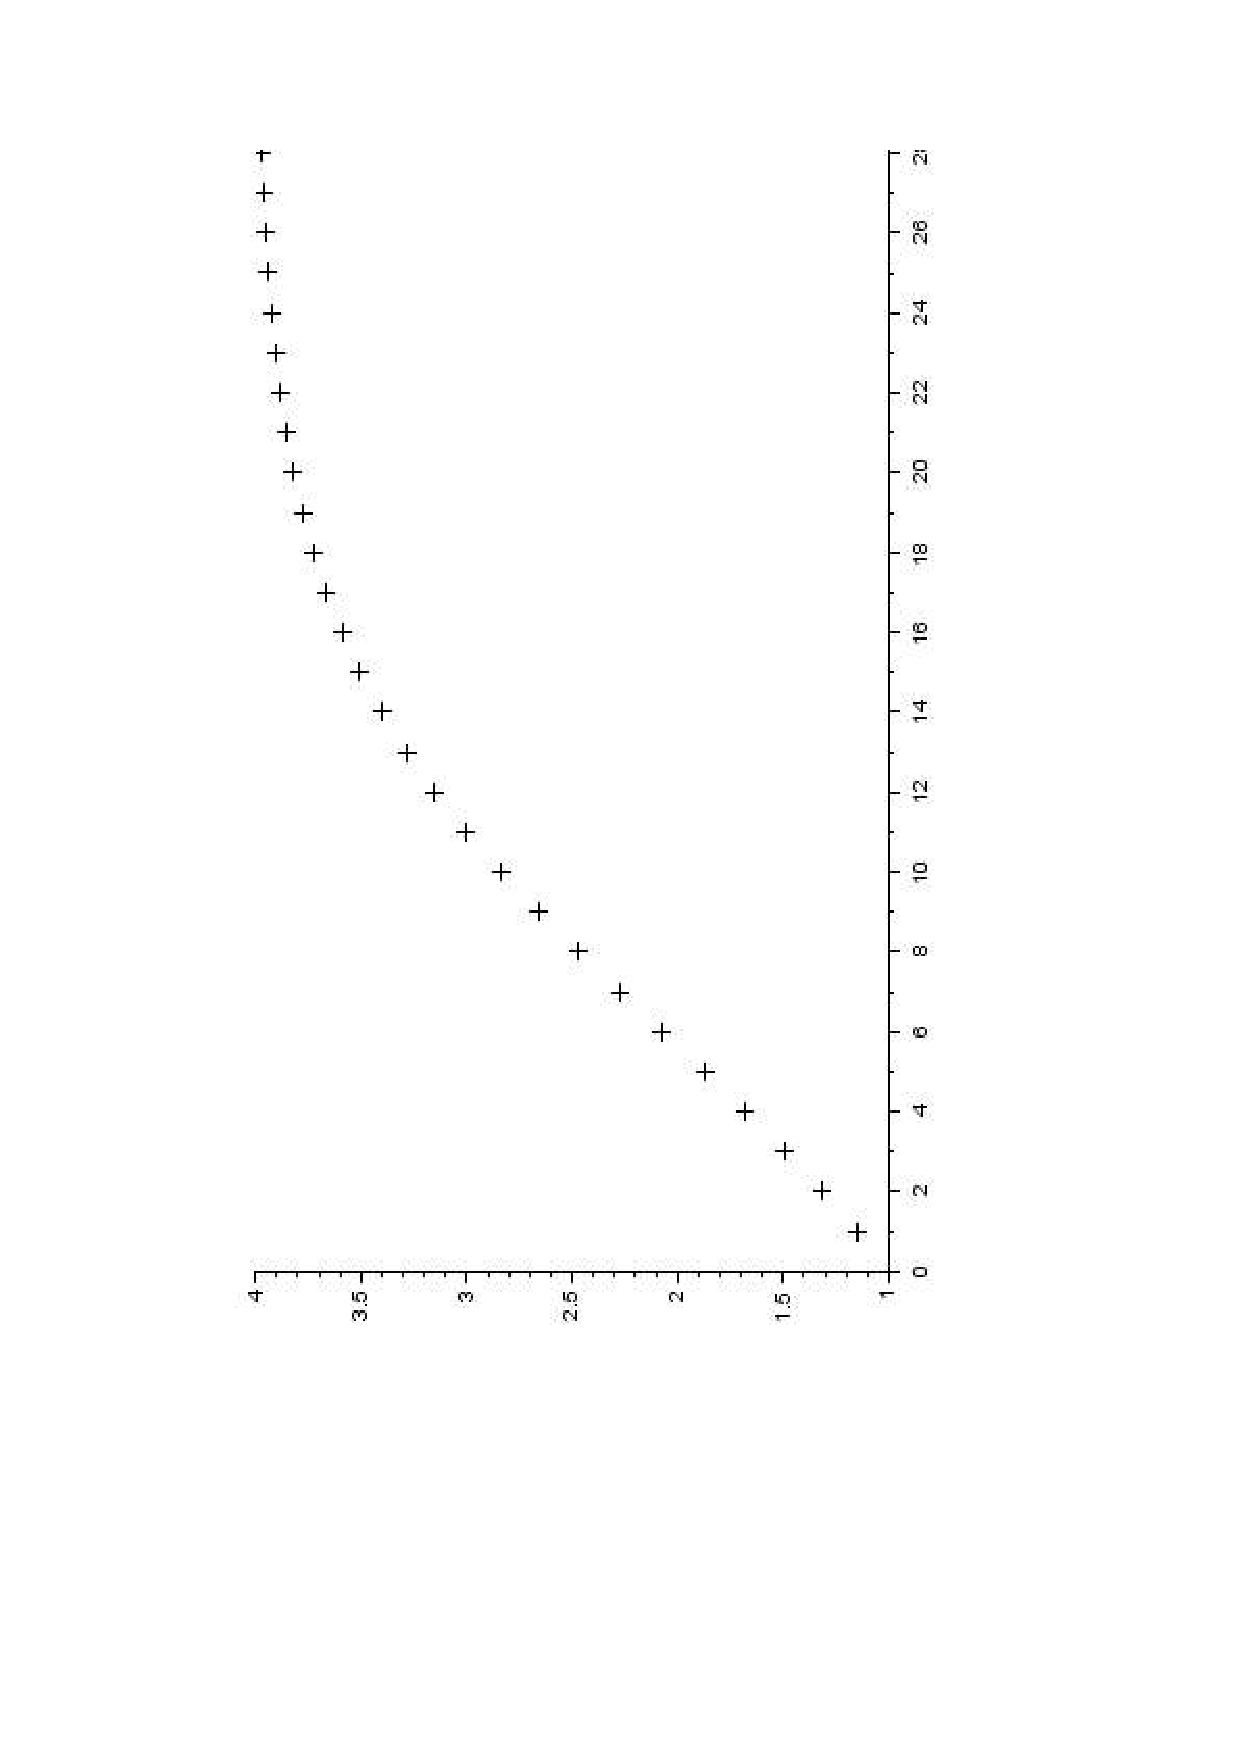
\includegraphics[width=300px]{logistique.png}
\end{center}
Paramètres de modélisation : $K=2$  ; $r=0.4$ 
\paragraph{}

\newpage

\paragraph{Discrétisation du modèle}
\begin{center}
%\includegraphics[width=300px]{discretisation.png}
\end{center}
Paramètres de modélisation : $a=1$ ; $h=0.1$ ; $K=2$  ; $r=0.4$
\paragraph{}

\subsubsection{Modèle avec variation de K}

\paragraph{Courbe de la vitesse d'accroissement}
\begin{center}
%\includegraphics[width=300px]{logistiqueR.png}
\end{center}
Paramètres de modélisation : $K=2$  ; $r$ varie de 0 à 1 avec un pas de 0.1
\paragraph{}

\paragraph{Discrétisation du modèle}
\begin{center}
%\includegraphics[width=300px]{discretisationR.png}
\end{center}
Paramètres de modélisation : $r=0.4$  ; $r$ varie de 1 à 1.6 avec un pas de 0.1
\paragraph{}

\subsubsection{Modèle avec variation de A}

\paragraph{Courbe de la vitesse d'accroissement}
\begin{center}
%\includegraphics[width=300px]{logistiqueK.png}
\end{center}
Paramètres de modélisation : $r=0.4$  ; $K$ varie de 1 à 1.6 avec un pas de 0.1
\paragraph{}

\paragraph{Discrétisation du modèle}
\begin{center}
%\includegraphics[width=300px]{discretisationK.png}
\end{center}
Paramètres de modélisation : $r=0.4$  ; $K$ varie de 1 à 1.6 avec un pas de 0.1
\paragraph{}

\subsubsection{Modèle avec variation de la population initiale}

\paragraph{Discretisation du modèle}
\begin{center}
%\includegraphics[width=300px]{discretisationK.png}
\end{center}


\newpage

\subsection{Etude mathématique}


\subsection{Bilan}
\paragraph{}

\newpage
\section{Etude du modèle logistique avec prédation}

\subsection{Etude numérique}

\subsubsection{Modèle logistique avec effet Allee}

\paragraph{Vitesse d'accroissement du modèle logistique sans / avec effet Allee}
\begin{center}
%\includegraphics[width=300px]{allee.png}
\end{center}
Paramètres de modélisation : $A=1$  ; $K=2$  ; $r=0.4$
\paragraph{}

\paragraph{Discretisation}
\begin{center}
%\includegraphics[width=300px]{discretisationAllee.png}
\end{center}
Paramètres de modélisation : $A=1$  ; $K=2$  ; $r=0.4$  ; $a = 1.2$ ; $h=0.1$
\paragraph{}

\subsubsection{Modèle logistique avec effet Allee avec variation de a}
\begin{center}
%\includegraphics[width=300px]{discretisationAlleea.PNG}
\end{center}
Paramètres de modélisation : $A=1$  ; $K=2$  ; $r=0.4$  ; $h=0.1$ ; $a$ varie de 0.5 à 2.5 avec un pas de 0.1
\paragraph{}

\subsubsection{Modèle logistique avec effet Allee avec variation de K}
\begin{center}
%\includegraphics[width=300px]{discretisationAlleeK.PNG}
\end{center}
Paramètres de modélisation : $A=1$  ; $a=1.2$  ; $r=0.4$  ; $h=0.1$ ; $K$ varie de 1.5 à 2.5 avec un pas de 0.1
\paragraph{}

\subsubsection{Modèle logistique avec effet Allee avec variation de A}
\begin{center}
%\includegraphics[width=300px]{discretisationAlleeSeuil.PNG}
\end{center}
Paramètres de modélisation : $K=2$  ; $a=1.2$  ; $r=0.4$  ; $h=0.1$ ; $A$ varie de 0.5 à 1.5 avec un pas de 0.1
\paragraph{}

\subsection{Etude mathématique}

\subsection{Bilan}
\paragraph{}


\newpage
\appendix

\section{Etude du modèle logistique avec effet Allee et immigration- Scripts Scilab}

\subsection{Modèle logitigue}

\subsubsection{Vitesse d'accroissement}

\begin{verbatim}
\end{verbatim}

\subsubsection{Discretisation}

\begin{verbatim}
\end{verbatim}

\subsection{Modèle logistique avec variation de r}

\subsubsection{Vitesse d'accroissement}

\begin{verbatim}
\end{verbatim}

\subsubsection{Discretisation}

\begin{verbatim}
\end{verbatim}

\subsection{Modèle logistique avec variation de K}

\subsubsection{Vitesse d'accroissement}

\begin{verbatim}
\end{verbatim}

\subsubsection{Discretisation}

\begin{verbatim}
\end{verbatim}

\section{Etude du modèle logistique avec prédation - Scripts Scilab}

\subsection{Modèle logistique}

\subsubsection{Vitesse d'accroissements du modèle logistique sans / avec effet Allee}

\begin{verbatim}
\end{verbatim}

\subsubsection{Discretisation}

\begin{verbatim}
\end{verbatim}

\subsection{Modèle logistique}

\begin{verbatim}
\end{verbatim}

\subsection{Modèle logistique}

\begin{verbatim}
\end{verbatim}

\subsection{Modèle logistique}

\begin{verbatim}
\end{verbatim}

\end{document}